\begin{refsegment}
	\chapter{Contexte biologique et méthodologique}

    Ce chapitre présente les notions biologiques puis informatiques, utilisées comme fondement du travail de recherche effectué lors de cette thèse.
    
    
    \section{Le métabolisme et sa représentation informatique}
    \subsection{Généralités sur le métabolisme}
    
    Pour perpétuer son espèce, tout organisme vivant consomme de l'énergie pour produire de la biomasse et se répliquer. Pour cela, l'être vivant doit assimiler des composés présent dans son environnement. Ces composés chimiques permettent de produire l'énergie, nécessaire à la survie mais surtout à la transmission du patrimoine génétique. Ainsi on désigne par métabolisme, l'ensemble des processus de synthèse et dégradation de composés chimiques, mis en œuvre par l'organisme. De fait, les processus comme la réplication de l'\gls{ADN}, la traduction d'un gène et autres \ldots~sont exclus.
    
    \note{Le mot métabolisme à évolué à travers l'histoire pour nous parvenir sous ça forme actuelle. En grec ancien on utilise "\greekFont{μεταβολή}" équivalent à metabolé désignant "transformation". Le mot métabole signifie "qui subit un changement". Il a été utilisé par la suite comme mot racine: métabol-ique, métabol-isme \ldots
    }
    
    Les organismes vivant opèrent une multitude de transformations chimiques. Ils forment de véritable usine de traitement biochimique. En effet, ils disposent d'une batterie de réaction biochimique, afin de traiter un grand nombre de composés, tant à l'intérieur qu'à l'extérieur de la cellule. Par exemple, certains composés, de par la nature de la membrane cellulaire \footnote{La membrane cellulaire constitue une barrière physique entre le milieu extérieur et intérieur de la cellule.}, doivent être transformé depuis l'extérieur de la cellule, afin d'assimiler le composé transformé. De ce fait, la matière présente dans l'environnement est utilisé pour constituer les briques nécessaires au vivant.
    
    Par conséquent, le métabolisme est essentiel à la vie, d'une part il fournit l'énergie nécessaire. Et d'autre part, il va produire les molécules de base indispensables à l'organisme, pour sa construction, sa défense et autres \ldots
    
    Bien qu'agissant à une échelle moléculaire, le métabolisme d'un groupe d'organisme peut impacter son environnement. Si bien que les conséquences peuvent être observées à l'échelle humaine voire dans certains cas à l'échelle de la planète (voir Figure~\ref{fig:bloom}). Un autre exemple est celui des espèces végétales. Ils absorbent du dioxyde de carbone et produisent de l'oxygène. Ainsi ils jouent un rôle important dans la concentration de ces composés dans l’atmosphère.
    
    
    \begin{shadedfigure}
        \begin{subfigure}[b]{.5\textwidth}
            \centering
            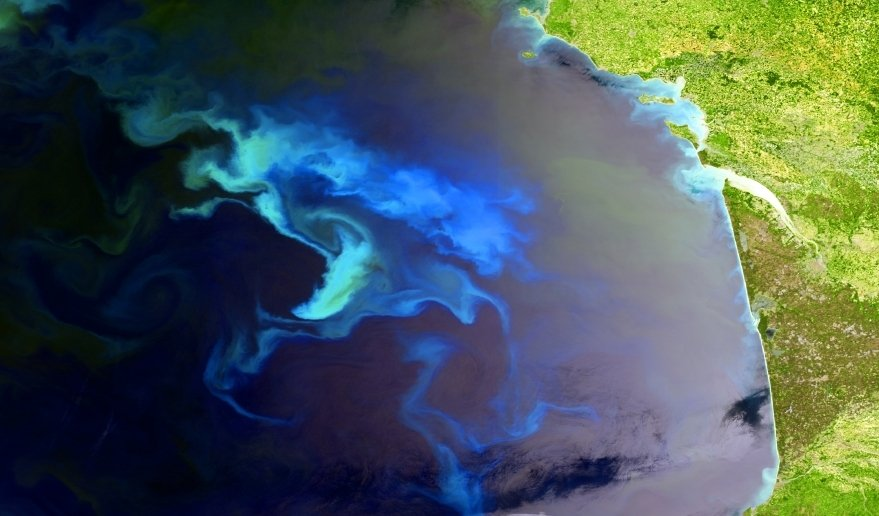
\includegraphics[width=\textwidth]{img/bloom_gascogne.jpg}
            \caption{{\tiny Source: \url{http://seos-project.eu}}}
            \label{fig:bloom_gascogne}
        \end{subfigure}
        \hfill
        \begin{subfigure}[b]{.5\textwidth}
            \centering
            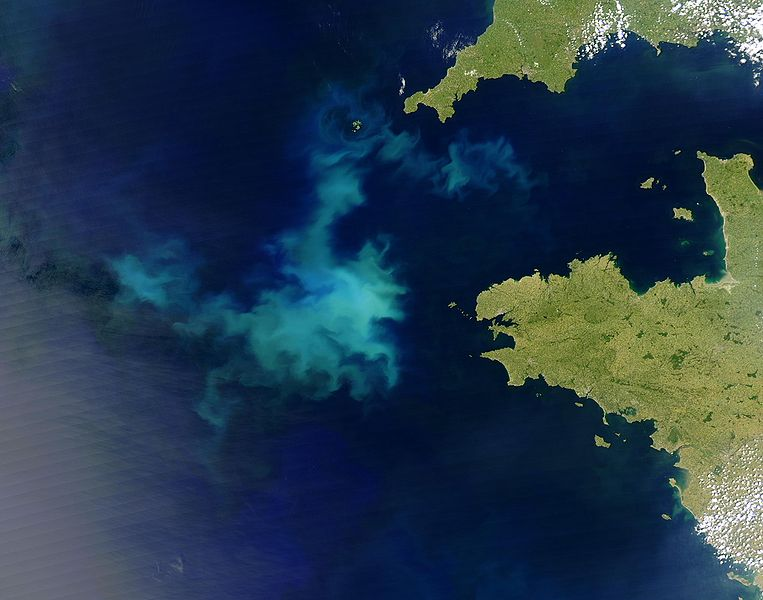
\includegraphics[width=\textwidth]{img/bloom_bretagne.jpg}
            \caption{{\tiny Source: \url{https://commons.wikimedia.org/}}}
            \label{fig:bloom_bretagne}
        \end{subfigure}
        \caption{Le métabolisme d'un groupe d'individu produit une quantité de pigment photosynthétiques suffisamment conséquente, qu'il en devient observable depuis l'espace. Deux évènements distincts sont représentés. Le premier a eu lieu au large de la Gascogne le 17 mai 2004 et le second au niveau de la Bretagne le 15 juin 2004.}
        \label{fig:bloom}
    \end{shadedfigure}
    
    \note{Lors de l'apparition des premières formes de vie, il y a 3,6 milliards d’années. L'atmosphère était faiblement pourvue en oxygène. Ces organismes anaérobiques était présent dans les océans. L'oxygène est toxique, leur métabolisme s'est adapté au dioxyde de carbone, présent abondamment à ce moment. Puis entre 3,5 à 3 milliards apparurent des cyanobactéries. Ce sont des bactéries capable de capter l'énergie du soleil. Elles sont "photosynthétiques". Leurs métabolismes possèdent la particularité d'oxyder les minéraux présents dans les océans. Ils produisent ainsi de l'oxygène. Avec le temps leur métabolisme a consommé tellement de minéraux que l'oxygène produits dans les océans s’est libéré dans l’atmosphère. Modifiant ainsi fortement sa composition. Cet évènement influença le cours de la vie. De sorte que des organismes s'adaptent à l'oxygène. Car l'oxygène devient alors une molécule courante. Certaine forme de vie évolua jusqu'à devenir aérobie. Avec cet évènement, la Terre a subi sa première pollution atmosphérique d'ampleur induit par des organismes vivant. (Lire: \citetitle{bengtson1994early} ) }
    

    \subsection{Les acteurs}
    
    L'étude du métabolisme est essentiel pour la compréhension des êtres vivants. Les débouchés impactent de nombreux domaines, tel que : la pharmaceutique, l'énergie, l'agriculture, l'environnement\ldots.  Pour mieux le comprendre, il est nécessaire d'introduire les différents acteurs du métabolisme. En effet, le métabolisme représente un ensemble d'événement faisant intervenir des métabolites, des réactions, des cofacteurs, des enzymes\ldots.
    
    
    
    \subsubsection{Les métabolites}
    
    Ce sont des composés organiques, de petites tailles, produits à travers les différents processus issus du métabolisme. Ils sont tour à tour synthétisés puis dégradés. Selon leurs rôles, ils interviennent soit dans les processus indispensables au développement et à la reproduction, dit "métabolisme primaire" . Soit pour des fonctions, non vitale comme la production d'antibiotique, de phéromone, de pigment \ldots, dénommé "métabolisme secondaire" .
    
    \note{Un composé organique s'oppose à un composé minéral. Cette différenciation s'explique par des raisons philosophiques antérieur au \siecle{19}. En effet, on distinguait les substances constitutives des organismes des autres. Ne sachant pas synthétiser les molécules organiques. On expliquait que l'intervention d'une "force vitale" était nécessaire. En 1828, Friedrich Wöler mis au point, accidentellement une expérience, produisant de l'urée (considéré comme organique) à partir de composé minéraux, comme le cyanate d’ammonium. Depuis lors, la notion de composé organique a évolué afin de désigner une molécule constituée d'une partie de carbone, le reste pouvant être des atomes d'hydrogène, oxygène azote et autres \ldots. La notion organique est resté car le carbone est un élément essentiel du vivant. Par opposition un composé minéral correspond à toutes molécules constituées d'élément autre que le carbone. Pour plus d'information, je vous invite à lire \citetitle{chimie_organique}.
    }    
      

	\subsubsection{Les réactions}
	Le processus de transformation d’un métabolite est décrit par une réaction. On désigne par le terme "substrat", les métabolites avant transformation. Par opposition, on parle de produit pour la molécule transformée. Ainsi une réaction est l'événement qui va transformer un substrat afin de produire un nouveau métabolite. Ces réactions s'effectuent au sein de l'organisme, dans l'infiniment petit, au niveau moléculaire.
    
    Une réaction est généralement représentée, par l’addition des molécules nécessaires à la transformation d’un côté. Puis de l’autre côté on expose la somme des molécules produites (voir figure \ref{fig:reaction}). Cette équation  représente la stœchiométrie de la réaction. C’est-à-dire que la proportion des éléments en jeu avant et après la réaction est respectée. De tels réactions sont représentées à l'équilibre, c'est-à-dire que la proportion de chaque atome est identique entre avant et après la réaction. Pour reprendre la célèbre maxime "Rien ne se perd, rien ne se crée, tout se transforme" .
    
    \begin{shadedfigure}
        \centering
        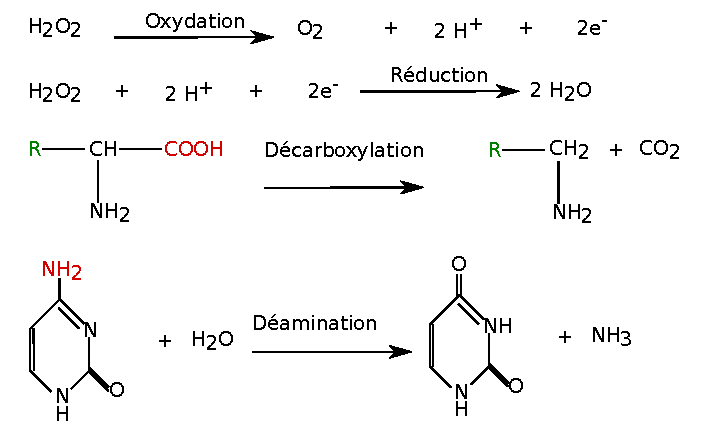
\includegraphics[width=\textwidth]{img/equation_reaction.pdf}
        \caption{Représentation de réaction sous leur forme "équation-bilan" .}
        \label{fig:reaction}
    \end{shadedfigure}
    
    \citation{ On voit que, pour arriver à la solution de ces deux questions, il fallait d'abord bien connaître l'analyse et la nature du corps susceptible de fermenter, et les produits de la fermentation ; car rien ne se crée, ni dans les opérations de l'art, ni dans celles de la nature, et l'on peut poser en principe que, dans toute opération, il y a une égale quantité de matière avant et après l'opération ; que la qualité et la quantité des principes est la même, et qu'il n'y a que des changements, des modifications }{Antoine Lavoisier}[Traité élémentaire de chimie, 1864]
    
    
    \subsubsection{Les enzymes}    
    La plupart de ces transformations ne sont pas spontanées où se feraient trop lentement. Pour cela, l'organisme dispose de molécule protéique facilitant ces transformations, appelé "enzyme". Ce sont des bio-catalyseurs, c'est-à-dire qu'elles vont favoriser ou accélérer une transformation chimique. Ces molécules peuvent couper, coller, réparer synthétiser ou encore modifier une molécule. Elles ont la particularité d'avoir une forte affinité avec leur substrat.  Leur rencontre provoque une transformation du composé. Puis, le ou les produits résultant de cette transformations, peuvent êtres à leur tour reconnu par d'autres enzymes. Provoquant ainsi une cascade de transformation chimique. 
    
    Une enzyme est une molécule constituée d'acide aminé, dont sa structure tri-dimensionnel contient des régions impliquées dans la reconnaissance et la transformation d’une molécule. C'est pourquoi, une même enzyme reconnaît une ou plusieurs molécules spécifiquement et induit les mêmes transformations chimiques. Ce processus est décrit par le modèle de "clef / serrure" (voir figure \ref{fig:reaction_enzymatique}). Le plus couramment les enzymes sont répertoriées selon quatre numéros séparé par des points désignant la réaction chimique qu'elles catalysent. C'est le système de nomenclature \gls{EC}. Chaque nombre est associé à un concept. Ainsi le premier indique le type de réaction catalysé,  le second décrit la catégorie du substrat utilisé, le troisième correspond au substrat spécifiquement impliqué et enfin le quatrième le numéro de série de l'enzyme.
    
    \begin{shadedfigure}
        \centering
        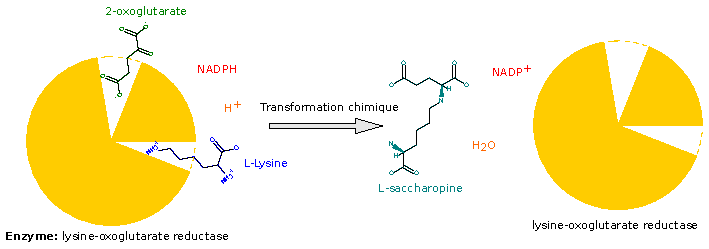
\includegraphics[width=\textwidth]{img/lysine-oxoglutarate_reductase.pdf}
        \caption{Schéma d'une réaction chimique catalysée par une enzyme. L'enzyme reconnaît ces substrats 2-oxoglutarate et L-Lysine, puis les transforme en une molécule de L-Saccharopine. La molécule NADPH$^{+}$ est nécessaire à l'activité enzymatique. On parle de cofacteur.}
        \label{fig:reaction_enzymatique}
    \end{shadedfigure}
    
    Une enzyme possède une affinité importante avec son substrat. Cette affinité influe sur l’activité enzymatique, c’est-à-dire sur la vitesse de transformation du substrat. Il existe des molécules, autres que les substrats de l’enzyme,  avec  une forte affinité pour l’enzyme. De tels molécules vont diminuer l’activité enzymatique. Les inhibiteurs enzymatiques joue un rôle important dans le métabolisme. Ils sont employés comme régulateurs du métabolisme. 
    
    \note{
        Les inhibiteurs enzymatiques permettent de limiter voir d’arrêter l’activité d’une enzyme. Cette caractéristique est employée pour  tuer des organismes pathogènes. Par exemple, La Pénicilline est un inhibiteur de la  transpeptidase intervenant dans la synthèse du peptidoglycane. Le peptidoglycane forme la paroi des bactéries. Si cette dernière est dans l’incapacité de synthétiser ça paroi alors cela conduit à la mort de la bactérie.
    }

    \subsubsection{Les cofacteurs}
    Certaines réactions nécessitent l’apport d'énergie, d’ion ou encore de molécules d'assistance qui vont favoriser l’activité enzymatique. \textbf{(trop brut pas de liaison)} Les enzymes nécessitant l'apport de cofacteur sont appelées holoenzyme lorsque le cofacteur est liée à cette dernière. Par opposition une enzyme inactive non lié à son cofacteur est une apoenzyme. Les cofacteurs sont classifiés en deux catégories : les ions métalliques et les coenzymes.
    
    Les ions métalliques de par leurs charges positives permettent de contre-balancer les charges négatives, amener soit par les chaines d'histidines de l'enzyme soit lors de la réaction catalytique \cite{christianson1991structural}. Dans le premier cas l'ion métallique joue un rôle structural au sein de l'enzyme. Dans le second il va assister l'enzyme dans son processus de transformation tout en maintenant sa structure. Effectivement les ions métalliques de part leur nature peuvent assister l'enzyme lors des réactions d'oxydoréduction et de transfert d'électron. Les ions fréquemment observé dans le vivant sont les ions fers, cuivres, zincs et magnésiums.
    
    Les coenzymes sont des molécules organiques. Elles sont rangées en deux groupes en fonction de la nature de la liaison établie avec l'apoenzyme.
    
    Le premier groupe contient les cofacteurs liés faiblement à l'enzyme. Ces cofacteurs subissent généralement une transformation lors de la réaction. Pour cette raison ils sont également appelé co-substrat. Par exemple une des réactions de la glycolyse implique le cofacteur NADP$^{+}$ pour transformer le glucose-6-phosphate (voir \ref{eq:glucose}). Ce cofacteur  se lie à l'enzyme puis il est transformé au cours de la réaction en NADPH. Cette modification engendre la libération du cofacteur de l'enzyme. Ce groupe contient également des cofacteurs énergétiques, c'est-à-dire que la transformation du cofacteur va engendrer une libération d'énergie. Cette énergie permet de réaliser des transformations qui était dans la cellule énergétiquement défavorable. De nombreux mécanismes essentiels au vivant nécessite l'apport d'énergie. Pour ces raisons le métabolisme d'un organisme est adapté à son environnement afin de produire l'énergie indispensable à sa survie et sa reproduction. Majoritairement le nucléotide \gls{ATP} est utilisé par le vivant comme cofacteur énergétique. L'hydrolyse de l'\gls{ATP} en \gls{ADP} induit la coupure d'une liaison avec un phosphate provoquant une libération d'énergie. On retrouve également d'autres cofacteurs utilisant la guanine, la thymine, la cytosine ou encore l'uracile en lieu et place de l'adénine (respectivement  GTP, TTP, CTP et UTP ). Le vivant est en perpétuel déséquilibre énergétique de part les différents processus qui le constitue, l'apport énergétique permet le maintien de la vie.
    
    \begin{equation}\label{eq:glucose}
        glucose-6-phosphate + NADP^{+} \rightarrow 6-phosphoglucono-D-lactone + NADPH + H^{+}
        \stepcounter{equation}\tag{équation \theequation}
    \end{equation}
    
    Le deuxième groupe de coenzyme représente les cofacteurs liés de façon covalente \footnote{Une liaison covalente est une liaison chimique dans laquelle deux atomes sont mutuellement attirer par une force. Cette force provient de la mise en commun d'au moins un électron par atome.} à l'enzyme. Ils sont appelés "groupements prosthétiques". Un des exemples les plus connu et celui de l'hème des hématies. C'est un groupement contenant un atome de métal (souvent le fer) permettant de capturer un gaz diatomique comme le dioxygène (O${2}$) où encore le monoxyde de carbone (CO).
    
    Ainsi le vivant via ces différents acteurs possèdent des combinaisons de réactions lui procurant les moyens de vivre et de se reproduire. Ces successions de réactions sont humainement représentées selon des objectifs considérés d'intérêts biologiques. Pour cette raison un cheminement de transformation métabolique en métabolique est appelé "voie métabolique".
    
    
    \subsubsection{Voies métaboliques}
    On distingue dans le métabolisme deux catégories de processus, l'anabolisme et le catabolisme. L'anabolisme, représente l'ensemble des réactions impliqué dans la synthèse de nouvelle molécule. La production de nouveaux composés nécessite de l'énergie. De tels processus sont constitués de réaction endergonique. Ainsi le bilan énergétique est négatif.  Au contraire, le catabolisme décrit l'ensemble des réactions de dégradation de molécule. Les réactions impliquées dans la dégradation d'une composé, produisent in-fine plus d'énergie qu'elles en on consommé. Ces réactions produisant de l'énergie sont dites exergoniques.
    
    Ces notions permettent de diviser l'ensemble des processus du métabolisme en sous-parties plus faciles à appréhender. Toujours dans l'intention de réduire l'énorme quantité de concept. Les réactions sont regroupées dans différentes entités appelées "voie métabolique". Ce découpage permet de représenter des segments d'évènement de transformation métabolique en ensemble de réaction permettant de réaliser un objectif d'intérêt biologique. Certains objectifs peuvent être atteints par des successions de réactions différentes. Ainsi une même voie métabolique peut être réalisé par différents chemins de réaction.
    
    Étant donnée que ces modules métaboliques réalise des transformations apportant un avantage à la cellule. Ces modules via le principe de pression de sélection vont tendre à garder la même structuration \cite{braakman2012compositional}. Les gènes correspondant aux protéines impliquées dans ces voies sont souvent co-localisées sur le génome. En effet une telle disposition des gènes favorise l'expression de toutes les protéines nécessaires pour la réalisation de l'objectif biologique à un instant "\textit{t}". De tels dispositions simplifie le processus de régulation d'expressions de ces gènes. Ce qui se traduit souvent par un gain énergétique donc un avantage évolutif pour la cellule. Comprendre la structuration du métabolisme, c'est également expliquer comment la physique et la chimie ont contraint la vie et l'évolution.
    
    Ces voies métaboliques sont des réactions connectées les unes aux autres. Ils se représentent intuitivement sous forme de graphe.
    
    \subsection{Représentation en graphe}
    
    De tels représentations permettent de partager des notions complexes sur un grand nombre de concepts ainsi que leurs relations. Les graphes s'avèrent utile pour l'étude des divers réseaux. Par exemple, le réseau routier, ça représentation est intuitive et permet la mise œuvre d'algorithme de recherche du plus court chemin. Cette branche des mathématiques s'est illustrer à travers la résolution  de problème complexe comme la traversée des sept ponts de Königsberg, la marche du cavalier sur l’échiquier et bien d'autres. Les applications des recherches issue de la théorie des graphes sont multiples. On retrouve son utilisation dans des domaines comme la chimie, le stockage de donnée (à travers les bases de données type graphe), l'ontologie (et ces relations entre les concepts), la biologie et ces différents réseaux (dont le métabolisme). Cette représentation de l'information à montrer son utilité à des problèmes complexe très variés.
    
    Avant d'aller plus loin, il est nécessaire de définir plusieurs notions employées dans la théorie des graphes. Tout d'abord un graphe est constitué de nœud relié entre eux. Les nœuds du graphe sont également appelés sommets ("vertice" en anglais).  Lorsque les relations indique un sens de cheminement entre deux nœuds ("edge" en anglais), elles sont qualifiés d'arc autrement on parle d'arrête. Ainsi on fait la distinction en graphe orienté et non-orienté. Généralement un graphe est désigné sous la forme mathématique :
    
    \begin{equation}\label{eq:graph}
    	G = (V,E) \stepcounter{equation}\tag{équation \theequation}
    \end{equation}
    
    Dans l'\ref{eq:graph}, G désigne le graphe tel que constitué de deux ensembles, celui des sommets V et celui des relations V. Différents type de graphe sont présentés dans la figure  \ref{fig:graphe}.
    
    
    \begin{shadedfigure}
    	\centering
    	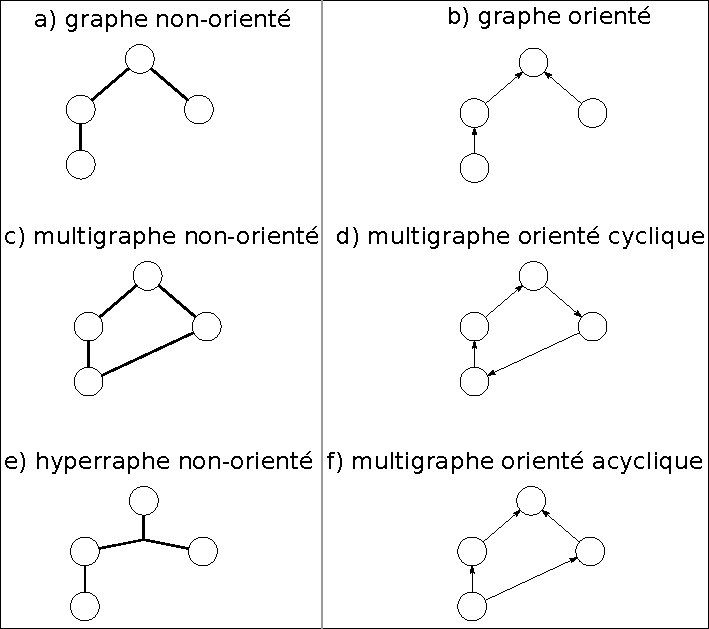
\includegraphics[width=\textwidth]{img/graph.pdf}
    	\caption{a) un graphe  avec des arrêtes. b) Un graphe avec des arcs indiquant une orientation entre deux sommets. c) un multigraphe non orienté avec des arêtes reliant les deux mêmes sommets. d) un multigraphe dont les relations forme un chemin cyclique à travers les sommets. e) un graphe avec une hyperarête reliant deux sommets. f) un multigraphe avec une orientation des relations tels que le chemin à travers le graphe traverse qu'une seule fois les sommets. }
    	\label{fig:graphe}
    \end{shadedfigure}
    
    
    
    Dans le cadre de la biologie, de nombreux évènements se représentent sous forme de réseaux. Pour en citer quelques uns, il y a les réseaux : d'interactions physiques protéine-protéine, de régulation de l'expression des gènes, de maximisation de flux (\gls{FBA}), de réaction métabolique… 
    
    Dans ce chapitre allons nous intéresser à la représentation en graphe des voie métaboliques. 
    
    \subsection{Ressources sur les voies métaboliques}
    
    Une voie métabolique est un enchainement de réaction enzymatique durant lequel les métabolites sont transformés. Ils représentent usuellement une fonction biologique. Par conséquent ces fonctions sont susceptibles d'être partagés à travers le monde du vivant. Toutefois pour réaliser une fonction biologique, il peut exister plusieurs variantes de chemin réactionnel. Par exemple pour la biosynthèse de la L-lysine, six voies alternatives sont connus à ce jour dans le monde du vivant (voir Figure \ref{fig:lysine} ).
    	
    	
    	\begin{shadedfigure}
    		\centering
    		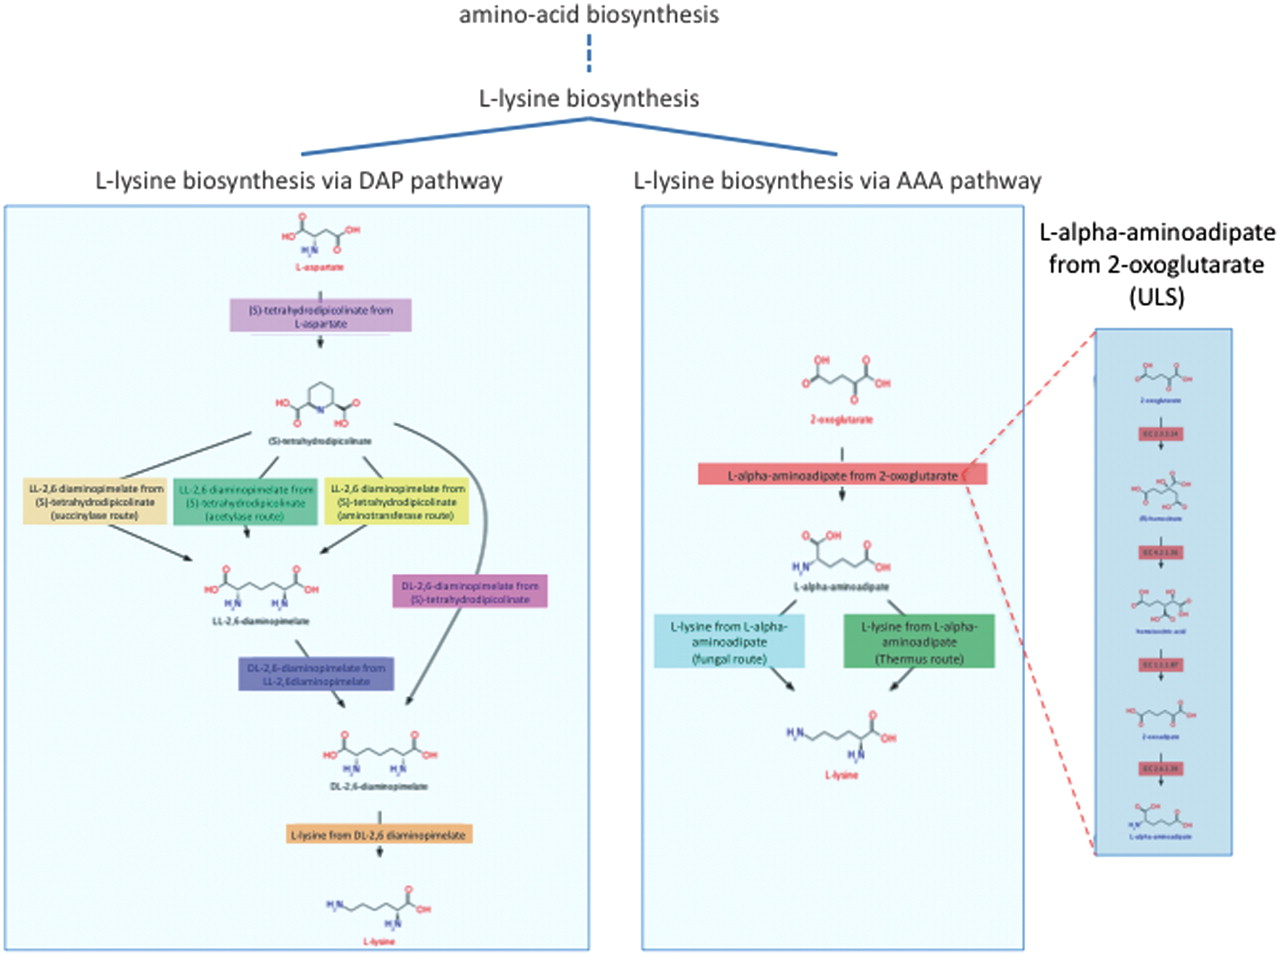
\includegraphics[width=\textwidth]{img/L-lysine-biosynthesis.jpg}
    		\caption{Biosynthèse de la L-Lysine peut se faire par via la voie DAP et ses quatre chemins de réactions possibles où via la voie AAA et ces deux voies alternatives. Figure reprise de l'article \citetitle{morgat2011unipathway}. }
    		\label{fig:lysine}
    	\end{shadedfigure}
     
     La représentation des voies métaboliques est une synthèse d'évènements se produisant le vivant. Par conséquent cette représentation est subjective. Elle diffère selon les éléments souhaitais être en avant où bien encore selon les informations et les meta-informations dont dispose la ressource. Ces différences seront exposées à travers les ressources sur les voies métaboliques KEGG, Reactome, Unipathway, Genome properties.
     
    \subsubsection{KEGG}
    
    La ressource KEGG (pour \textit{Kyoto Encyclopedia of genes and Genomes}) \cite{ogata1999kegg,kanehisa2000kegg,kanehisa2002kegg,kanehisa2004kegg,aoki2005using,kanehisa2010kegg,kanehisa2017kegg} organise le réseau métabolique en un graphe dirigé (voir Figure \ref{fig:kegg_lysine}). Ce réseau est découpé sous forme de carte répertoriant toutes les réactions supposées avoir lieu dans le domaine du vivant. La construction de ce réseau provient essentiellement de prédiction bio-informatique.
    
    \begin{shadedfigure}
        \centering
        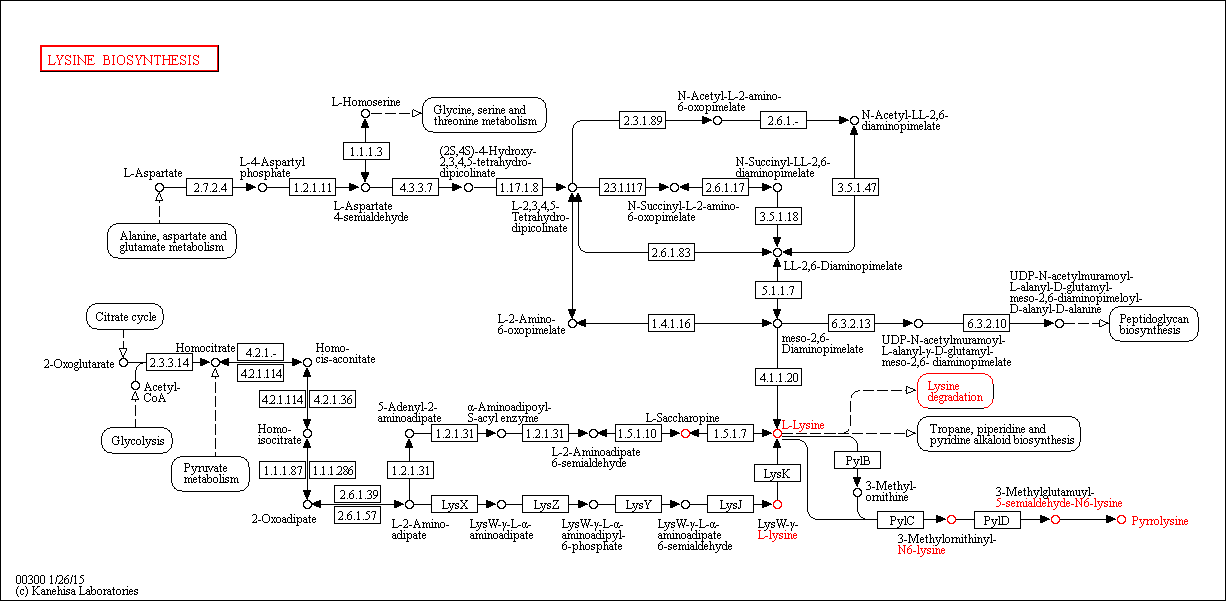
\includegraphics[width=\textwidth]{img/kegg_lysine.png}
        \caption{ Représentation du réseau métabolique selon un graphe dirigé. Les sommets du graphe sont des métabolites et les arcs correspondent aux réactions. Carte extraite de la ressource en ligne "KEGG pathway". }
        \label{fig:kegg_lysine}
    \end{shadedfigure}
    
    \subsubsection{Reactome}
    Le projet Reactome \cite{joshi2005reactome,matthews2009reactome,croft2010reactome,croft2014reactome,fabregat2016reactome} met à la disposition de la communauté des voies métaboliques expertisées et vérifiées par l'Homme. Différentes vues sont proposées selon le niveau hiérarchique du concept sélectionné (voir Figure \ref{fig:reactome_metabolism} et \ref{fig:reactome_serine}). Cette ressource contient à ce jour 19 organismes eucaryotes. La curation puis l'organisation des données est couteuse en temps. Pour ce donner un ordre d'idée sur l'avancement du travail d'expertise et d'intégration la version 54 de septembre 2015 comprenait 43\% des gènes humains. Ceci représente un total de 8701 gènes sur les 20 296 gènes codant pour des protéines prédits.
    
    \begin{shadedfigure}
        \begin{subfigure}[t]{.5\textwidth}
            \centering
            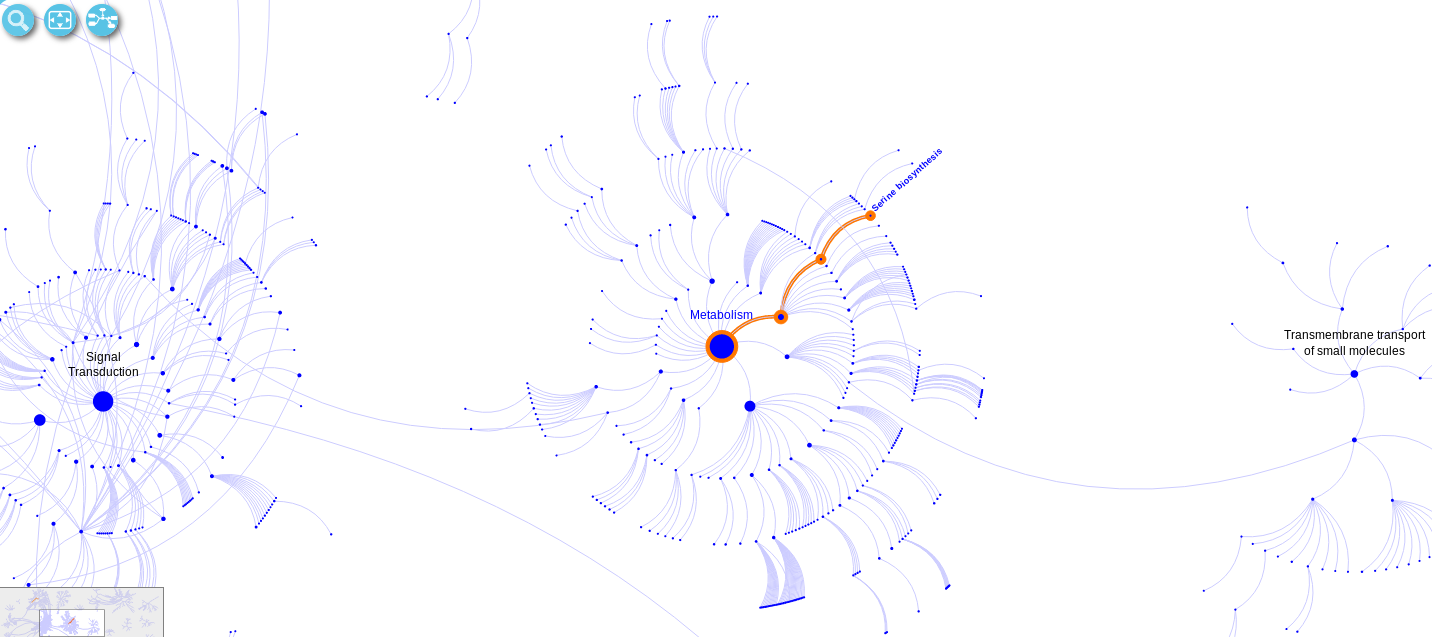
\includegraphics[angle=90,origin=c,width=\textwidth]{img/reactome_homo_sapiens_metabolism.png}
            \caption{ Vue globale des relations ontologique chez l'Homme sous forme de graphe hiérarchique. En naviguant du centre vers l'extrémité des sous-graphes, les concepts vont des plus généraux aux plus spécifiques. }
            \label{fig:reactome_metabolism}
        \end{subfigure}
    \hfill
    \begin{subfigure}[t]{.45\textwidth}
        \centering
        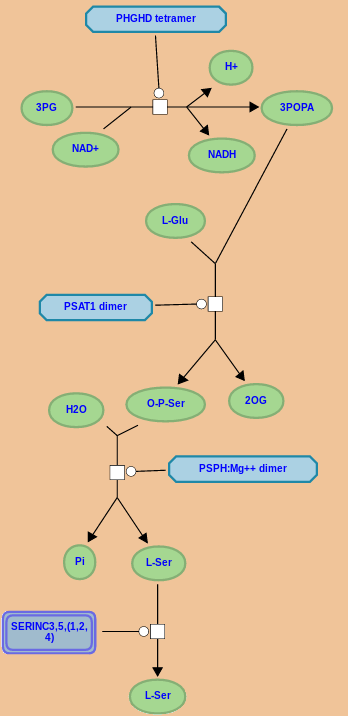
\includegraphics[width=\textwidth]{img/reactome_homo_sapiens_serine_biosynthesis.png}
        \caption{ Représentation du réseau métabolique selon un hypergraphe dirigé. Les sommets verts sont les métabolites et cofacteur participants à la réaction. Les réactions correspondent aux sommets représenté par des carrés blancs. Les sommets cerclés de bleu sont les étiquettes attachées à la réaction, afin d'indiquer le nom de l'enzyme, le numéro \gls{EC} de la réaction et autres informations\ldots. Les hyperarêtes indique le sens de la réaction et pointes sur les molécules transformées. }
        \label{fig:reactome_serine}
    \end{subfigure}
    \end{shadedfigure}

    \subsubsection{Unipathway}
    
    Cette ressource en ligne fournissait un travail de curation des voies métaboliques \cite{morgat2011unipathway}. C'est-à-dire qu'il y avait une validation des voies métaboliques prédites par de l'expérimentation et/ou de l'expertise humaine. Le réseau métabolique est découpé en cinq concepts, les voies métaboliques (\gls{UPA}), les chemins réactionnels linéaires (\gls{ULS}), les réactions enzymatiques (\gls{UER}), les réactions chimiques (\gls{UCR}) , les composés (\gls{UPC}) (voir Figure \ref{fig:unipathway_structure}). Ces concepts sont ordonnés les uns par rapport aux autres via des relations de compositions et d'équivalence. Le modèle est très flexible il fait une distinction entre réaction chimique et réaction enzymatique. En effet une réaction chimique peut être spontané et/ou être réalisé par différent bio-catalyseur. Enfin à travers le concept d'\gls{ULS}, la ressource fait apparaître les enchainements de réactions permettant de réaliser un objectif biologique. Un \gls{ULS} est un ensemble réaction (\gls{UER}) impliqué dans une seule tâche biologique. Ainsi les \gls{ULS} comprenant plusieurs réactions, sont délimités par des réactions impliquée dans au moins deux processus biologiques. Cependant, il est très fréquent de voir une même réaction impliquée dans plusieurs processus biologiques. C'est pourquoi seulement 30\% des \gls{ULS} ont plus de deux réactions. Toutefois un incident technique a provoqué l'arrêt de ce projet. Cette base d'information est encore à ce jour indisponible : \url{http://www.unipathway.org/}.
    
    \note{
    	Selon le fournisseur d'internet néozélandais "\textit{Actrix}":
    	\begin{itemize}
    		\item 60\% des compagnies ayant perdu toutes leurs données ont fermé dans les 6 mois après l'évènement.
    		\item Il est estimé pour une heure de travail les données perdues coûte en moyenne à une entreprise 790 \$.
    		\item 31\% de la perte de donnée de plus de 500 000 \$ est due à une défaillance du système.
    		\item Un disque dur sur cinq est bloqué au cours de sa vie.
    	\end{itemize}
    	{\tiny Source: \url{http://editor.actrix.co.nz/0305.htm}.}
    }
    
    
    \begin{shadedfigure}
        \centering
        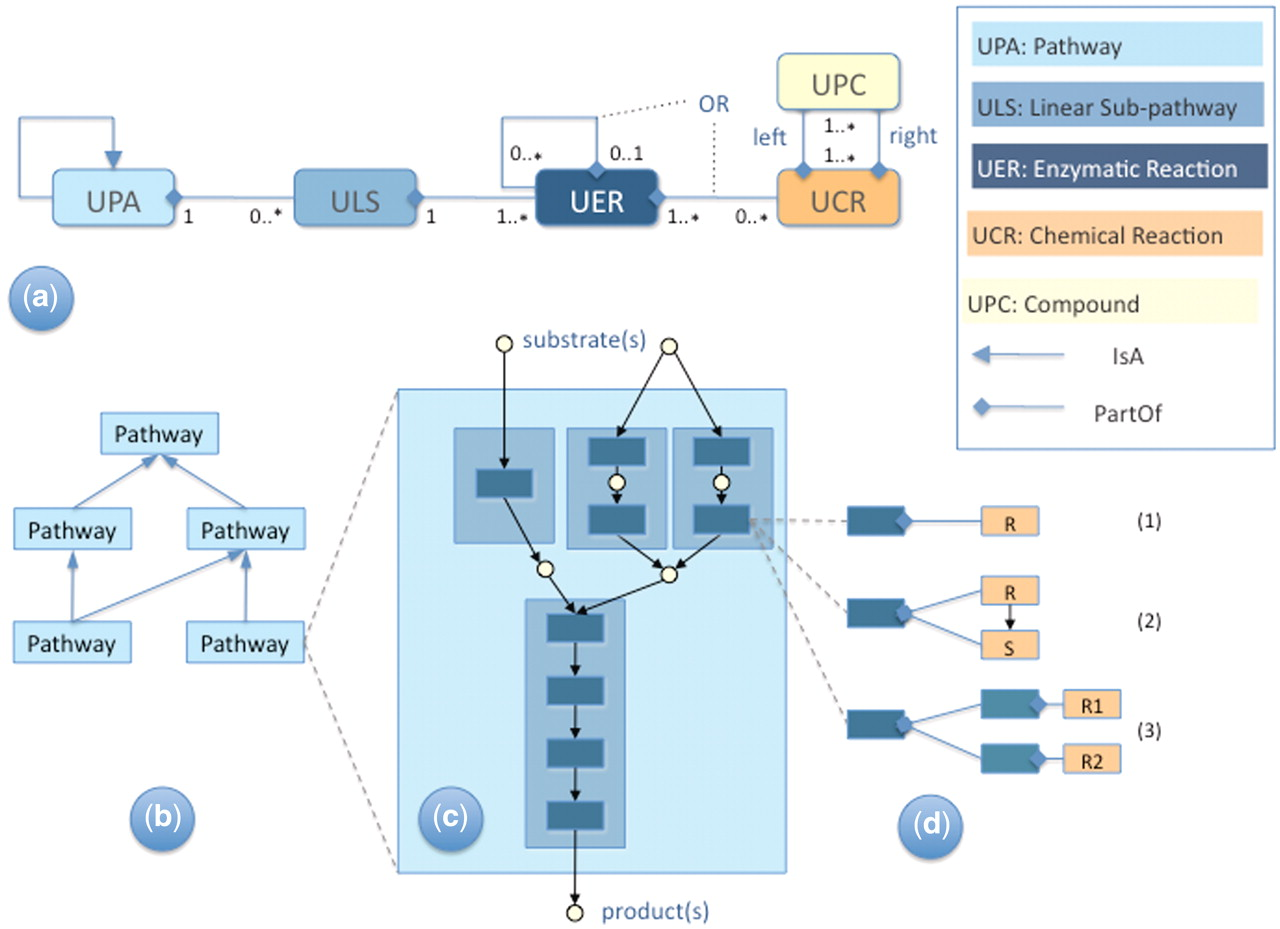
\includegraphics[width=\textwidth]{img/unipathway_structure.jpeg}
        \caption{ Overview of the UniPathway concepts. (a) Unified Modeling Language (UML)-like representation of the UniPathway classes and relationships. Legend is to the right of the main part of the figure. Multiplicity constraints read as: One UPA is composed of 0 or more ULS—One ULS is contained in exactly 1 UPA. One ULS is composed of 1 or more UER—One UER is contained in exactly 1 ULS. One UER is composed of 0 or more (alternate) UER—One UER is contained in 0 or at most 1 UER. One UER is composed of 0 or more UCR—One UCR is contained in 1 or more UER. One UCR is composed of 1 or more left UPC and 1 or more right UPC—One UPC is contained in 1 or more UCR. (b) Example of the IsA relationship defining the UniPathway controlled vocabulary hierarchy of pathway terms. A pathway instance may be a specific type of an abstract pathway entity. (c) Example of the PartOf relationship linking a pathway (UPA: light blue), its subpathways (ULS: blue) and individual enzymatic reactions that constitute the subpathway (UER: dark blue). (d) Three cases of the relationship between an UER and its chemical reaction components (UCR): (1) simple one-to-one relationship where R is catalyzed by a single enzyme; (2) R is catalyzed by an enzyme and S is a spontaneous reaction; (3) ‘OR’ relationship: the enzyme can catalyze two reactions differing by their co-substrates (e.g. NADH/NADPH).}
        \label{fig:unipathway_structure}
    \end{shadedfigure}

    \subsubsection{BioCyc et MetaCyc}
    
    \textit{BioCyc} \cite{caspi2006metacyc,caspi2007metacyc,caspi2008metacyc,caspi2010metacyc,caspi2012metacyc,caspi2013metacyc,caspi2014metacyc,caspi2015metacyc,caspi2016metacyc} est une collection en ligne (\url{https://biocyc.org/}) de voie métabolique et de génome (dénoté PGDBs pour "Pathway/Genome DataBases"). Cette resource fournit des données de qualtité à travers une sructure multi-couche afin d'avoir un panel d'information large et cohérent (voir Figure \ref{fig:biocyc_collection}) . Ajouté a ces données biologiques, BioCyc fournit des outils pour leurs explorations et compréhensions. Les PGDBs \textit{BioCyc} sont générées par un logiciel de prédiction des voies métaboliques nommé "PathwayTools" \cite{karpe2011pathway,karp2015pathway}. De plus il identifie les opérons \cite{romero2004using} et suggère des gènes pour les enzymes orphelines\footnote{Une enzyme est dites orpheline lorsque l'on n'est pas capable de l'associé à un gène.}\cite{Green2004}. \textit{BioCyc} intègre également les informations d'autres bases de données de bioinformatics, telles que les caractéristiques des protéines et l'information ontologique d'\textit{UniProt} portant sur les gènes . Le site Web \textit{BioCyc} offre une suite d'outils logiciels pour la recherche, l'analyse et la visualisation de donnée métabolique.
    
    
    \begin{shadedfigure}
    	\centering
    	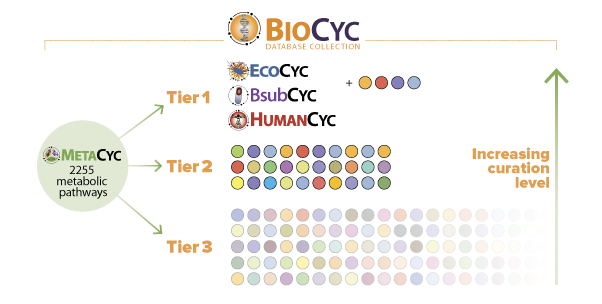
\includegraphics[width=\textwidth]{img/BioCycCollection.png}
    	\caption{\textit{BioCyc} est un ensemble de base de donnée et d'outil sur le métabolisme. \textit{Metacyc} regroupe l'ensemble des informations du monde vivant. Cette ressource comprend 2255 voies métaboliques à ce jour. Ces données biologiques sont répartis à travers 3 couches (i.e "Tiers"). Ces couches classifient le niveau de qualité des bases de données  (Du moins vers le plus qualitatif : tiers 3 à 1). \hspace{\textwidth} Source : \url{https://biocyc.org/}    }
    	\label{fig:biocyc_collection}
    \end{shadedfigure}
    
    \textit{MetaCyc} \cite{Karp2011,caspi2013metacyc,caspi2016metacyc} est une ressource universelle non redondante sur les voies métaboliques et les enzymes de tous le domaine du vivant. Cette ressource fournit des informations de qualité. Pour cela elle intègre seulement les voies métaboliques décrite dans la littérature scientifique et expérimentalement observées. Au sein du projet \textit{BioCyc} cette base de donnée est utilisé conjointement avec la partie \textit{PathoLogiC} de l'outil \textit{PathwayTools} pour la prédiction de voie métabolique de tout organisme complètement séquencé. 
    
    À travers les bases de données spécialisés sur un organisme comme \textit{EcoCyc} (\url{https://ecocyc.org/}) pour \textit{Escherichia coli}, \textit{BsubCyc} (\url{https://bsubcyc.org/}) pour \textit{Bacillus subtilis} ou encore \textit{HumanCyc} (\url{https://humancyc.org/}) pour l'Homme, BioCyc fournit une vue précise des informations sur l'organisme d'intérêt. Ceci est utile pour faire un bilan des connaissances accumulées au sein d'une espèce. Pour cela des outils dédiés viennent enrichir l'expérience utilisateur, comme la navigation dans le génome avec les annotations fonctionnelles sur les gènes (\url{https://ecocyc.org/ECOLI/select-gen-el}). On retrouve également une carte métabolique offrant une vue globale des connaissances métaboliques sur l'organisme (voir \url{https://bsubcyc.org/overviewsWeb/celOv.shtml} ). Ces données spécialisées peuvent être comparées aux autres organismes  (voir \url{https://humancyc.org/comp-genomics}) afin de mettre en évidences des connaissances communes (voir Tableau \ref{tab:compare_tools}).
    
    \begin{table}[H]
    	\caption{Extrait d'une analyse comparative sur les voies métaboliques communes entre d'\textit{Escherechia coli K-12 substr. MG1655}, \textit{Salmonella enterica enterica serovar Typhi str. CT18} et \textit{Shigella dysenteriae 1012} (requête: \url{https://ecocyc.org/comp-genomics?tables=pathway&orgids=\%28ECOLI+SENT220341+SDYS358708\%29}). }
    	\label{tab:compare_tools} 
    	\begin{tabular}{l|lll}
    		\toprule
    		Pathways Shared by Organism Pairs & Escherechia & Salmonella & Shigella \\
    		\midrule
    		Escherichia                       & 342         & 212        & 219      \\           
    		Salmonella                        & 212         & 341        & 274      \\           
    		Shigella                          & 219         & 274        & 335      \\ 
    		\bottomrule
    	\end{tabular}
    \end{table}
    
    
    Toutes ces données spécialisées sont croisées pour produire de la connaissance. Afin de visualiser ces connaissances \textit{Biocyc} met à disposition des tables de connaissances interactives, les "\gls{KS}" \cite{bat061SmartTable}. Ces tables intelligentes utilisent la représentation symbolique des connaissances. Elles permettent de regrouper les connaissances vis-à-vis de leur signification. Par exemple le groupe des "composés anti-tuberculosis  et leurs cibles dans  Mycobacterium tuberculosis H37Rv" est formé par l'analyse sémantique des données (voir le groupe : \url{https://biocyc.org/group?id=biocyc14-1553-3679321317}).
    
    
    
    
    \section{Des génomes aux réseaux métaboliques}
    
    La connaissance de l'origine des différentes protéines intervenant dans le métabolisme permet d'avoir un catalogue des capacités du vivant. Dès lors, il peut être réutilisé afin de prédire des fonctions métaboliques. Toutefois ce coût est rentabilisé car il deviendra utilisable pour rechercher sa présence dans tous les organismes. Afin d'aborder les liens entre le génome et le métabolisme d'un organisme, nous rappelons brièvement les trois niveaux qui les relient. Ceci implique :
    
    \begin{itemize}
        \item Le génome : composé d'un ensemble de gènes
        \item Le transcriptome : constitué d'\gls{ARNm} produit par l'organisme
        \item Le protéome : ensemble des protéines exprimées par l'organisme
    \end{itemize}
    
    \begin{shadedfigure}
        \centering
        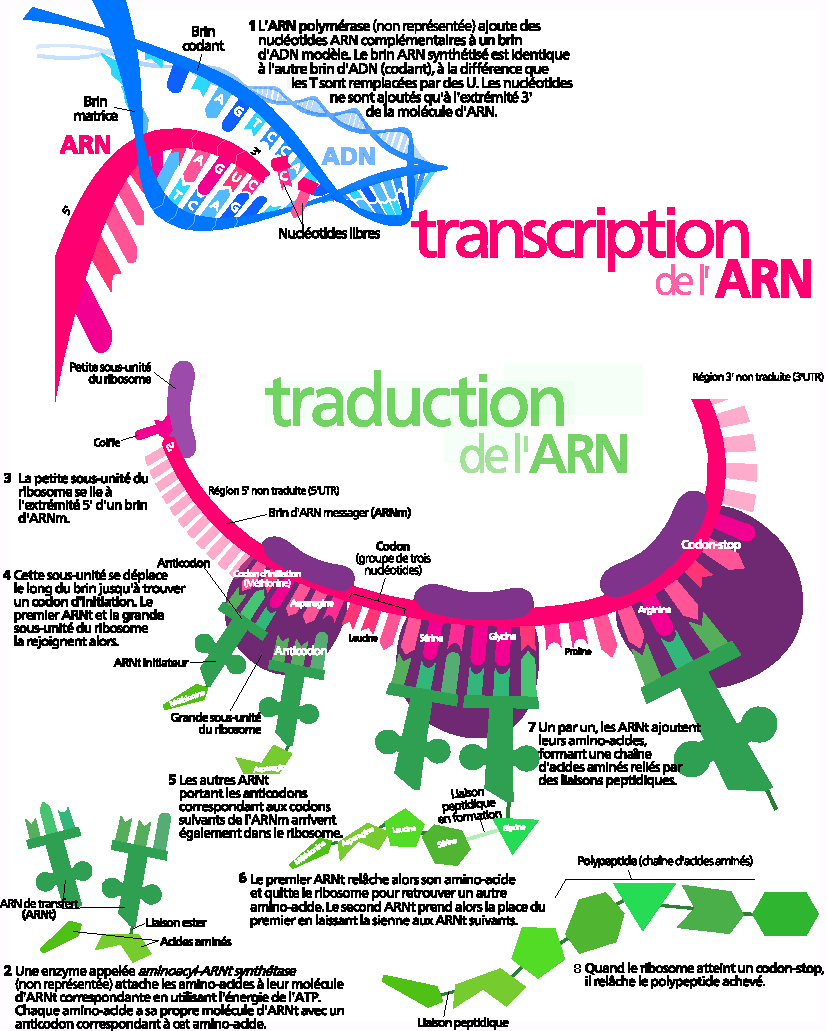
\includegraphics[width=\textwidth]{img/production_proteine2.pdf}
        \caption{Schéma des différentes étapes aboutissant à la production d’une protéine.}
        \label{fig:production_proteine}
    \end{shadedfigure}
    
    Le transcriptome et, dans un second temps, le protéome représentent les produits de l'expression des gènes. Ces deux niveaux sont dynamiques et changeant. Ils diffèrent selon les stress perçus par l'organisme. C'est-à-dire, à un temps donné, seulement une partie des gènes de l'organisme est exprimée. Alors que le génome d'un organisme est considéré comme invariant en gène. Ainsi pour chaque gène retrouvé dans un organisme, on sera en mesure de déterminer la ou les séquence(s) protéique(s) \footnote{Un même gène peut exprimer plusieurs protéines.}. Ce lien indirect entre le gène et protéine est également appelé "\acrshort{GPR}" pour : \textit{\acrfull{GPR}}.
    
    Afin de documenter le génome, le transcriptome et le protéome on passe par plusieurs étapes d’annotation. L’annotation peut être de nature automatique ou manuelle. Dans ce dernier cas, des experts vont effectuer un travail de validation et invalidation des annotations. Ce travail de curation des données est important car les prédicteurs automatiques ne sont pas toujours fiables.
    
    On distingue trois niveaux d’annotation pour un génome (Figure \ref{fig:niveaux_annotation}). Le premier niveau est l’annotation structurale. Elle est utilisée pour définir les bornes de début et de fin d’un gène.  Le second niveau est l’annotation fonctionnelle. Elle recherche à prédire les fonctions biologiques des gènes. Puis, le troisième niveau correspond à l’annotation relationnelle. Cette annotation consiste à étiqueter les différentes interactions entre les produits des gènes.
    
    \begin{shadedfigure}
        \centering
        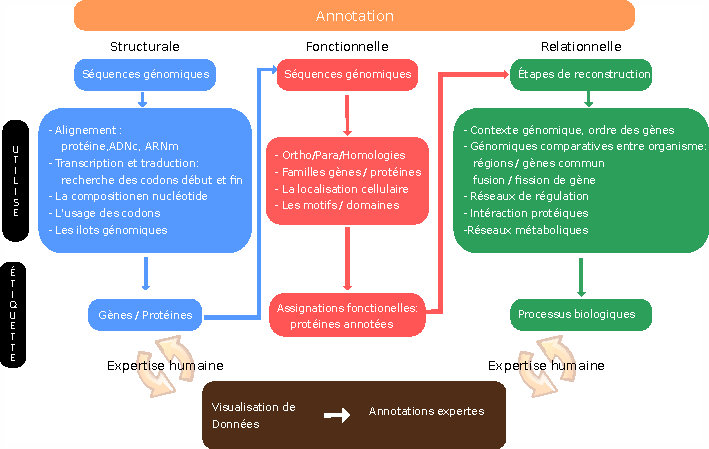
\includegraphics[width=\textwidth]{img/niveaux_annotations.pdf}
        \caption{Présentation des différents niveaux d’annotation.}
        \label{fig:niveaux_annotation}
    \end{shadedfigure}
    
    \subsection{L’évolution des génomes}
    Avant d'approfondir l’annotation génomique, il est nécessaire de comprendre le processus d’évolution des génomes. Car les méthodes d’annotation automatique utilisent cette théorie pour extrapoler des fonctionnalités d’un organisme vers un autre.
    
    Le principe explique que le vivant est soumis à différentes contraintes, environnementale par exemple ( ressources nutritives, température, acidité\ldots ), ainsi avec le temps les générations d’individus les plus adaptés à ces contraintes ont de meilleurs chances de se reproduirent. Par conséquent de transmettre leur patrimoine génétique. D’ailleurs c’est ce patrimoine génétique qui permet de s’adapter aux contraintes. Il est le support de l’expression métabolique et ce métabolisme peut fournir des avantages par rapport aux autres individus. Ainsi tant que métabolisme d’un organisme est adapté à ces contraintes, l’individu peut se reproduire et perpétuer sa lignée génétique.
    
    Toutefois le génome d’un enfant n’est pas forcément la copie exacte des parents. Différents évènements peuvent venir le modifier légèrement. Par conséquent les gènes modifiés vont produire une protéine légèrement différentes. Ces modifications peuvent alors soit procurer un avantage soit un désavantage qui va mener à la fin de la transmission de ce patrimoine. Pour cela, nous observons la plupart du temps seulement les organismes possédant un patrimoine génétique suffisamment adapté à leurs contraintes. En bref, les organismes sous l’effet de pression variées sont sélectionnées.
    
    Suivant cette théorie les gènes se modifient légèrement au cours du temps provoquant de légère modification de leurs séquences. Ainsi des séquences proche de par leur composition sont supposé effectuer produire des protéines avec des fonctions similaires. Le génome peut subir différents évènements qui vont conduire à l’expression de protéines différentes de l’origine. <- mal dit
    
    \begin{shadedfigure}
        \centering
        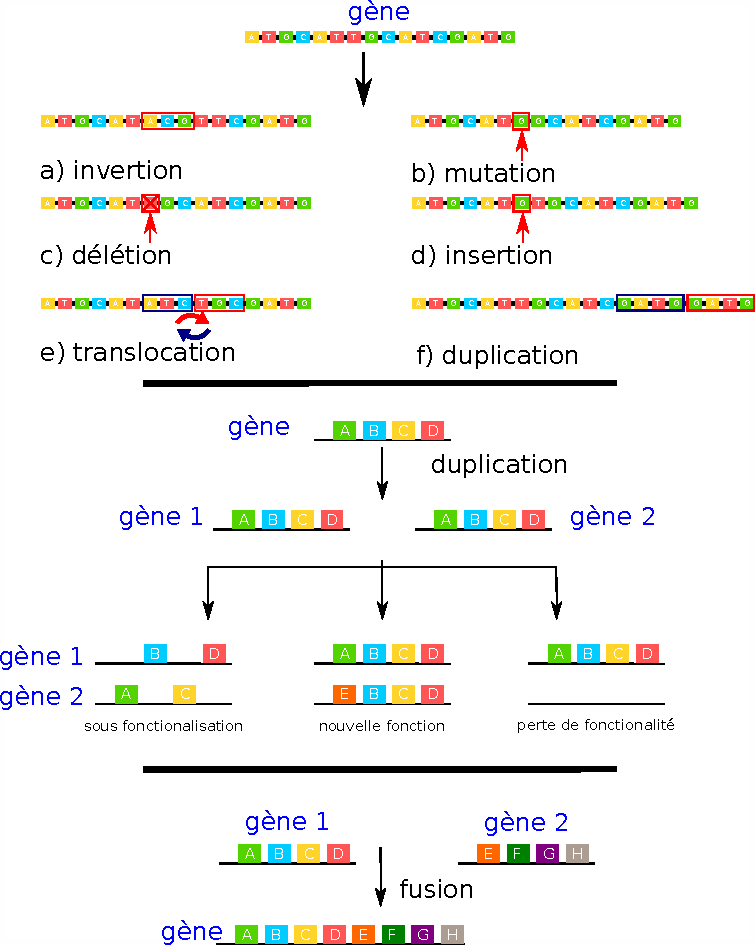
\includegraphics[width=\textwidth]{img/gene_indel.pdf}
        \caption{Présentation de plusieurs évènements génomiques....}
        \label{fig:/evenement_mutation}
    \end{shadedfigure}
    
    En conséquence, les gènes similaires d’organismes différents provenant d’un même gène ancestral sont dit homologues. Par contraste, les gènes d’organismes différents mais n’ayant pas la même origine sont définis comme analogue.
    
    Les évènements de duplications de gènes décrivent la création d’une nouvelle copie de gène dans l’organisme. Étant donné que l'organisme possède une fonctionnalité en double, une des copies peut diverger. En effet, il existe toujours la fonctionnalité originelle sur un gène. La pression de sélection implique qu’une des copies de gène produisent une protéine remplissant la même fonction originelle. On utilise le terme paralogue pour décrire des gènes issue de cet événement de duplication. Un tel évènement peut dupliquer un gène, une région de génome contenant plusieurs gènes  voir dans certains cas un génome.
    
    Les événements de fusion de gène représentent des gènes originellement séparé qui vont former un unique gène. Par opposition les évènements de fission vont  engendrer la coupure d’un gène en deux gènes distincts. Typiquement ce cas est observé avec des gènes codant pour des protéines multi-domaines. Par exemple, une protéine avec deux domaines, codé par un gène se fissure de tels sorte, que chacun des deux nouveaux gènes se spécialise pour produire un des deux domaines de la protéines. Ce phénomène peut engendrer une pression de sélection différentes sur ces deux gènes, selon l’importance du rôle joué par le domaine dans la protéine. Par conséquent un des deux gènes va diverger plus rapidement du gène ancestrale.
    
    Le relâchement de certains facteur de pression de sélection peut conduire à des événements de délétion. L’organisme n’étant plus contraint de posséder une fonctionnalité, les modifications du gène n’impacte pas la capacité de reproduction de l’organisme. Ces modifications peuvent amener à la disparition d’un gène fonctionnel. C’est-à-dire que la séquence du gène à garder des similarités avec le gène ancestrale mais il n’est plus en mesure de fournir la fonctionnalité.
    
    On retrouve également des évènements d’inversion de séquence, de translocations (le gène peut va être déplacé sur un autre chromosome), de transpositions ( un ou plusieurs gènes vont être directement intégré au sein du génome.
    
    L’accumulation de tous ces événements peuvent amener  à une divergence importante du génome par rapport à un génome ancestral. Ceci conduit à l’émergence de nouvelle espèce qui vont évoluer différemment. Ces espèces provenant d’une espèces ancestrales vont avoir des gènes proches. Ces gènes sont dits paralogues.
    
    L’horloge moléculaire des régions qui ne sont pas soumises à la pression de sélection naturelle (ne codant pas pour des gènes) et minimale dans les parties du génome soumises à une forte pression (c'est-à-dire les régions codant pour des fonctions essentielles à la survie de l'organisme).
    
    
    \subsection{Annotation des génomes}
    Changer le contenu de cette section car Annotation fonctionnelle est devenu annotation des génomes.
    Syntaxique, fonctionnelle, relationnelle (dont voies métaboliques) Zoom sur les fonctions impliquées dans les processus bio = voie métaboliques
    
    L’annotation fonctionnelle des gènes, correspond au processus d’attribution de rôle biologique à des gènes. En effet ces gènes vont produire des protéines disposant de une ou plusieurs fonctionnalités pour l’organisme. Ces fonctions sont habituellement classées en trois catégories : moléculaires, cellulaires, phénotypiques.
    
    Les fonctions moléculaires décrivent le rôle biochimique et/ou structural de la protéine. Ainsi les fonctionnalités de catalyse, de liaison et autres sont présentées.
    
    Les fonctions cellulaires établissent les différentes interactions de la protéines au sein de la cellule. Par exemple le rôle d’une enzyme dans une voie métabolique comme la biosynthèse de la lysine . 
    
    Les fonctions phénotypiques détails les caractéristiques observables induite par l’activité d’une protéine. A titre d’exemple, la présence ou l’absence d’une protéine peut jouer un rôle sur la capacité de l’organisme à se développer dans un environnement.
    
    Pour cela l’annotation fonctionnelle basé sur des méthodes expérimentales consiste à isoler chaque produit des gènes afin de tester leurs rôles. Par exemple on peut utiliser un vecteur de clonage contenant un gène d'intérêt. Puis on incorpore le vecteur de dans un organisme. Cet organisme est cultivé afin exprimer le gène d'intérêt. La protéine produit par le gène et ensuite purifier afin d'éliminer tout autre molécule. Et enfin seulement après la réussite des étapes précédentes, on va pouvoir tester les fonctions de la protéine.  Ces méthodes ne sont  pas envisageables à l’état d’un génome. Elles sont utilisées pour valider une prédiction bio-informatique.
    
    Les méthodes d’annotation fonctionnelles  bio-informatiques se base sur la comparaison de séquence. Ainsi les séquences homologues, les protéines de même familles, les séquences possédant un même domaine ou motif partageront des annotations fonctionnelles.
    
    \subsection{Reconstruction des réseaux métaboliques}
    Le métabolisme est un ensemble de réaction biochimique. Une réaction transforme des composés en de nouveaux métabolites. Ces derniers sont modifiés par d'autres transformations. Cette succession d'évènement peut être représenté sous la forme d’un graphe de réactions. Le produit d’une réaction est relié à une autre réaction lorsque cette dernière utilise ce métabolite transformé.
    
    
    \begin{shadedfigure}
        \centering
        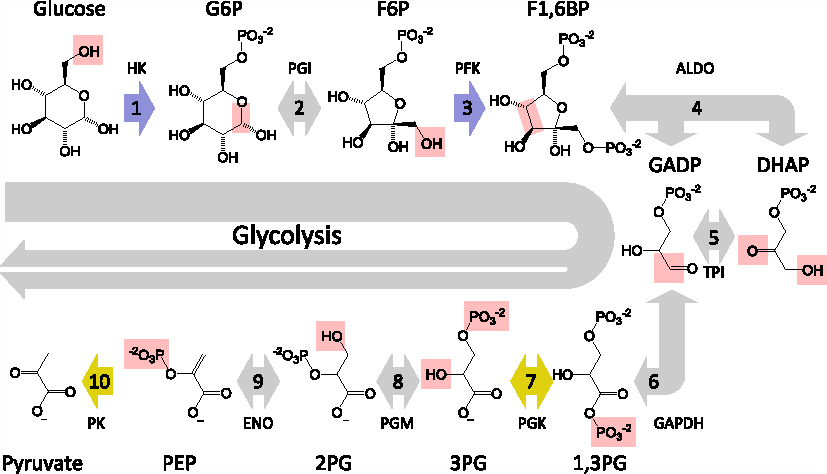
\includegraphics[width=\textwidth]{img/graphe_reactions_glycolyse.pdf}
        \caption{A changer source wikipedia.Représentation de la dégradation du glucose sous forme d’un graphe réactionnel. La  succession des réactions forme un chemin dans le réseau. Cette représentation a pour vocation de restreindre les évènements qui occurrent dans l'organisme aux réactions. Il est important de retenir que ce type de schéma, n'indique pas si ces réactions ont lieu dans le même compartiment cellulaire. Ou encore si les protéines nécessaires aux réactions sont toutes présentes à un moment donné. Cette une vue générale des réactions pouvant avoir lieu dans un organisme.  }
        \label{fig:glycolysis}
    \end{shadedfigure}

    \subsection{Modèles métaboliques}
    \subsection{Les données expérimentales}
    \subsubsection{Élucidation des voies métaboliques}
    Avec la découverte des enzymes à la fin du \siecle{19}, un nouveau champ de connaissance en biologie s’ouvrait. L’enzyme est la clé menant à la compréhension du vivant. Pour cela, la communauté scientifique réalisa un très grand nombre d’expérience permettant produire puis ...
    \subsubsection{Phénotypes de croissances}
    La plupart des molécules biologiques sont constituées d’atome de  carbone (C), d’hydrogène (H), d’oxygène (O), d’azote (N), de phosphore (P) et de soufre (S) (\acrshort{CHONPS}). Par conséquent les organismes doivent avoir au moins une source de nutrition pour chacun de ces éléments. En plus de ces éléments, on considère qu’il est nécessaire pour la vie d’avoir une source de potassium, de calcium, de magnésium, de fer, d’oligo-éléments et d’eau. Ce sont les éléments minimum pour la vie. Tout autres éléments permettant à des organismes de se développer est catégorisé comme facteur de croissance. 
    
    Selon les organismes vivants, leurs besoins en éléments et facteurs de croissances varient avec leur capacité métabolique. Ce qui permet de catégoriser les organismes, au regard des manières de constituer de la matière organique via leur anabolisme, ainsi que des moyens de production énergétique via leur catabolisme. (trop lourd) Ces catégories dites types trophiques dépendent de la nature  (i) de la source de carbone (ii) du donneur d’électrons (iii) de la source d'énergie (voir Tableau \ref{tab:type trophique}).
    \begin{landscape}
        \begin{table}[]
            \centering
            \caption{Structuration des différents types trophiques.}
            \label{tab:type trophique}
            \begin{tabular}{|l|l|lr|l|}
            	\hline
                \multirow{2}{*}{\specialcell{Lumière\\\textcolor{orange}{Photo}-}}    					      	&  \multirow{2}{*}{\specialcell{Composé organique\\-\textcolor{nicered}{organo}-}}  & Organique & -\textcolor{psviolet}{hétérotrophe} 	& \textcolor{orange}{Photo}\textcolor{nicered}{organo}\textcolor{psviolet}{hétérotrophe}    \\\cline{3-5}
                                                                                          					  	&                                                               					& Minérale 	& -\textcolor{bleudefrance}{autotrophe}	& \textcolor{orange}{Photo}\textcolor{nicered}{organo}\textcolor{bleudefrance}{autotrophe}  \\\cline{2-5}
                                                                                         					   	&  \multirow{2}{*}{\specialcell{Inorganique\\-\textcolor{brown}{litho}-}}           & Organique & -\textcolor{psviolet}{hétérotrophe} 	& \textcolor{orange}{Photo}\textcolor{brown}{litho}\textcolor{psviolet}{hétérotrophe}     	\\\cline{3-5}
                                                                                            					&                                                               					& Minérale 	& -\textcolor{bleudefrance}{autotrophe}	& \textcolor{orange}{Photo}\textcolor{brown}{litho}\textcolor{bleudefrance}{autotrophe}     \\ \hline
                \multirow{2}{*}{\specialcell{Composé chimique\\organique ou non\\\textcolor{vert}{Chimio}-}}  	&  \multirow{2}{*}{\specialcell{Composé organique\\-\textcolor{nicered}{organo}-}}  & Organique & -\textcolor{psviolet}{hétérotrophe} 	& \textcolor{vert}{Chimio}\textcolor{nicered}{organo}\textcolor{psviolet}{hétérotrophe}   	\\\cline{3-5}
                                                                                            					&                                                               					& Minérale 	& -\textcolor{bleudefrance}{autotrophe}	& \textcolor{vert}{Chimio}\textcolor{nicered}{organo}\textcolor{bleudefrance}{autotrophe}   \\\cline{2-5} 
                                                                                            					&  \multirow{2}{*}{\specialcell{Inorganique\\-\textcolor{brown}{litho}-}}           & Organique & -\textcolor{psviolet}{hétérotrophe} 	& \textcolor{vert}{Chimio}\textcolor{brown}{litho}\textcolor{psviolet}{hétérotrophe}    	\\\cline{3-5}
                                                                                            					&                                                               					& Minérale 	& -\textcolor{bleudefrance}{autotrophe}	& \textcolor{vert}{Chimio}\textcolor{brown}{litho}\textcolor{bleudefrance}{autotrophe}      \\ \hline
            \end{tabular}
        \end{table}
    \end{landscape}
    Certains organismes ont la faculté de se développer dans des milieux dépourvu de facteur de croissance. C’est-à-dire, qu'à partir des éléments minimaux nécessaires à la vie, ils sont capables de produire toutes les molécules  indispensables à leurs développement. Ce sont des organismes dit prototrophe.  Dans le cas contraire on parle d’auxotrophie. 
    
    Le métabolisme fournit les acides aminés indispensables à la production de protéines. Ces protéines sont constituées d’acides aminés. Par conséquent l’organisme doit se procurer ces acides aminés soit par des voies de biosynthèses soit directement par nutrition. C’est pour cela qu’avec les organismes prototrophes on s’attends à retrouver toutes les voies de la biosynthèses des acides aminés. Et par opposition un organisme auxotrophe à un acide aminé ne devrait pas avoir la voie de biosynthèse de ce dernier.
    
    \subsection{MicroScope : une plateforme d’annotation de génomes procaryotes et d’analyse de leur métabolisme}
    
    Chapeau : objectif MicroScope, les différentes publications
    Puis celle de 2017
    Section de la fin : souligner ce qui a été fait en terme de curation pour les bio… mais mieux à faire pour guider les bio dans leur travail de curati=> objectif de ton travail
    
    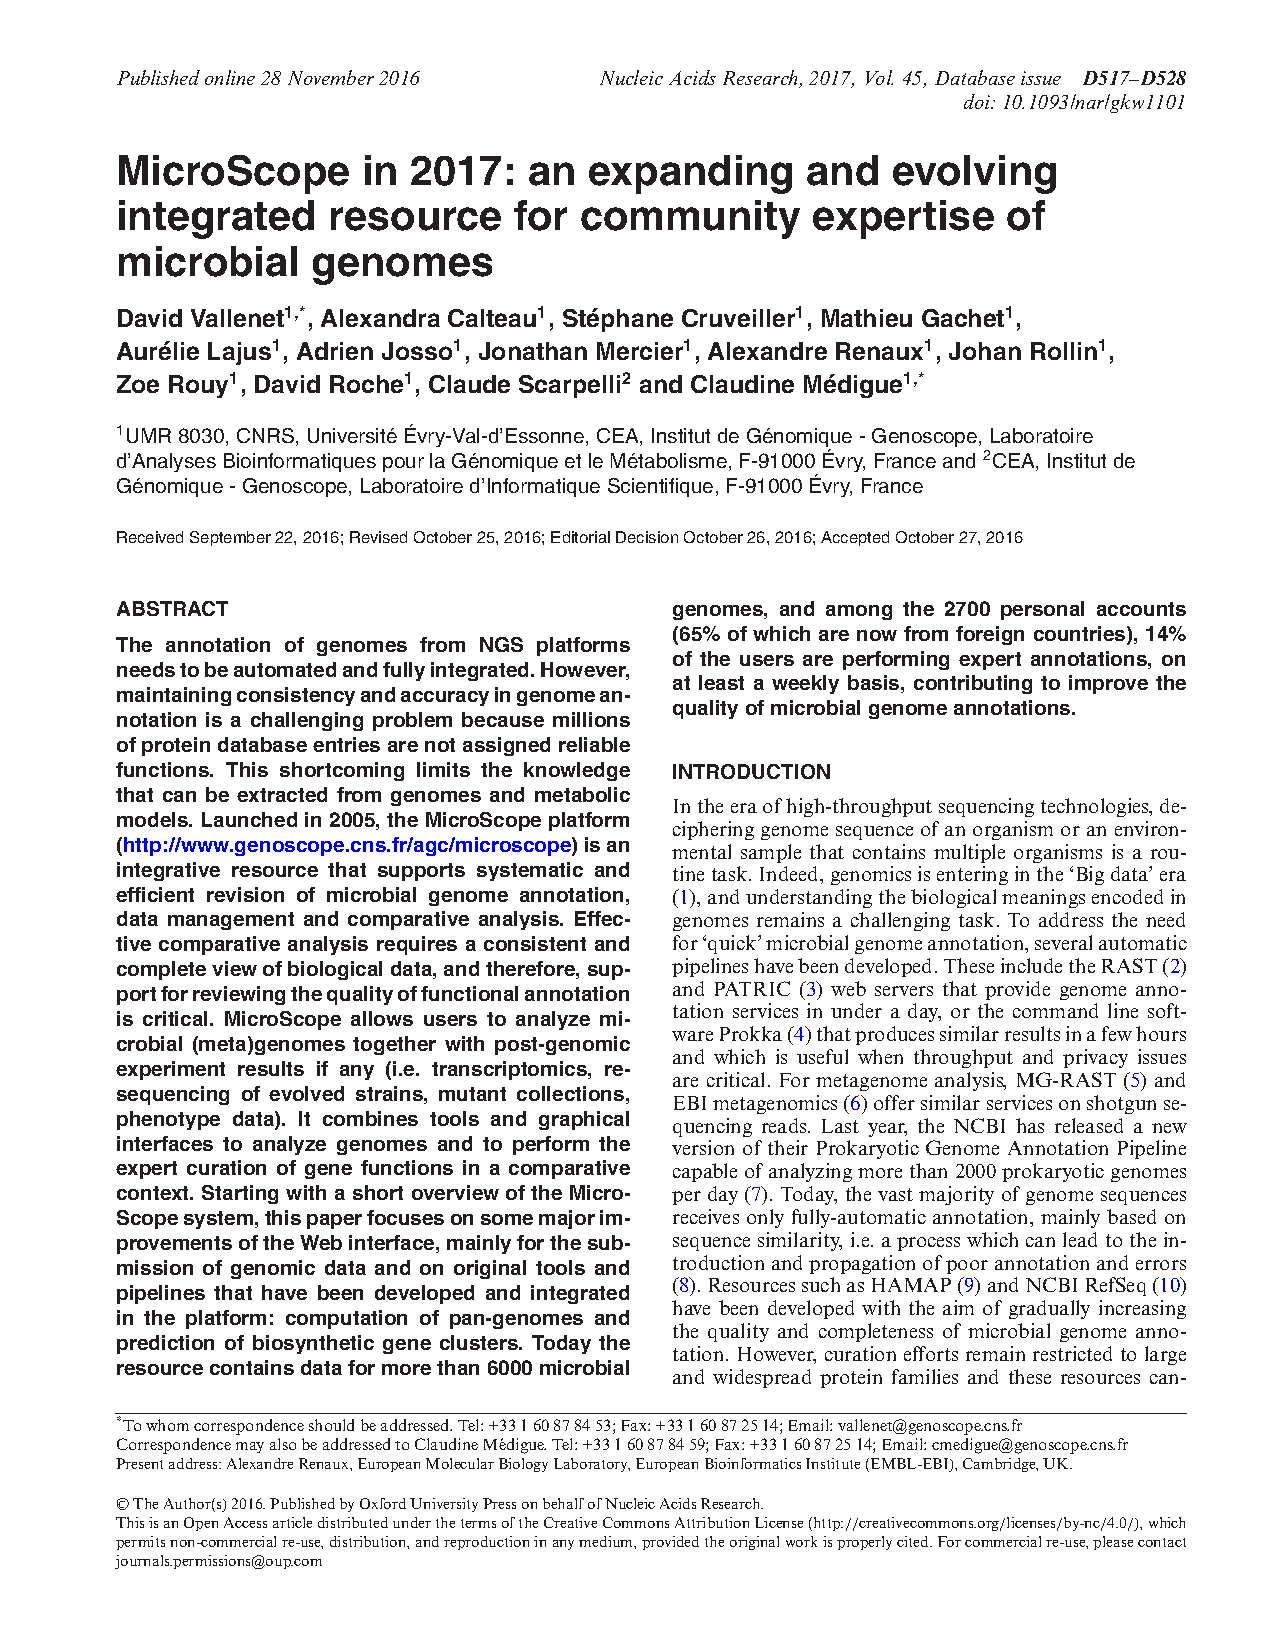
\includepdf[pages=-]{img/microscope2017.pdf}

    \section{Raisonnement logique dans le processus de curation}
    
    Le processus de curation consiste d’ajouter et/ou enlever des annotations manuellement. Pour cela les bio-curateurs utilisent un ensemble de règles qui leur sont propres. Une des méthodes utilisé par les bio-curateurs passe par la reconstruction des voies métaboliques. Le bio-curateur connaît des caractéristiques phénotypique de son organisme d’intérêt. Il va pour cela commencer par vérifier si les caractéristiques sont corrélés aux prédictions. Par exemple, lorsque l’on reconstruit les voies métaboliques d’un Citrobacter, on s’attend à retrouver au moins une voie complète, permettant la dégradation du citrate. Si ce n’est pas le cas, le bio-curateur informé de cette lacune dans l’annotation, va rechercher un ou plusieurs gènes permettant in-fine d’exprimer cette capacité.
    
    Par ailleurs, lorsque le bio-curateur s’aperçoit qu’il manque une réaction afin de réaliser une voie métabolique. Il va essayer de caractériser le gène en se basant sur le contexte génomique. Les gènes liés aux réactions qui précèdent et succèdent la réaction non annoté à un gène (trop compliqué)
    
    \subsection{Lacunes et incertitudes dans nos connaissances}
    
    Quelque soit le domaine d’expertise, nous avons des éléments imprédictibles par les modèles scientifiques. Notre savoir sur le monde qui nous entoure est encore partiel. Les modèles scientifiques permettent de représenter une partie de ce monde. Mais il existe un nombre de fait, non négligeable, qui échappe à ces  modèles. Ces trous de connaissances peuvent être identifiés lorsque l’on oppose les prédictions aux expectations. Il apparaît que des faits attendues reste non prédit.
    
    D’autre part, les ressources entreposant les faits prédits sont variées. Leurs prédictions proviennent  de différents algorithmes dont leur spécificité \footnote{Proportion de résultat négatifs correctement identifiés.} et sensibilité \footnote{Proportion de résultat positifs correctement identifiés.} diffèrent d’un algorithme à un autre. Ces prédictions aux taux d’erreurs variés viennent enrichir les entrepôts de données. Puis ils seront utilisé à leur tour utilisé pour prédire de nouveau faits. Par conséquent  le taux d’erreur de la première prédiction vient s’ajouter au taux d’erreur de la méthode. Ce processus cyclique, permet de capturer un nombre plus important de fait. Mais il a l’inconvénient de sur-prédire.
    
    Ces problématiques sont retrouvées dans le processus de prédictions de fonction protéiques.
    Pour pallier à ce phénomène des initiatives tente de limiter l’extrapolation abusive faites par les prédicteurs. Par exemple \citeauthor{pfeiffer2015manual}
    
    
    \subsubsection{Les trous dans les connaissances et les enzymes orphelines}
    \subsubsection{Limites de l’annotation fonctionnelle et rôle de la curation}
    \subsection{Logique et raisonnement}
    \subsubsection{Les différentes logiques}
    \paragraph{Logique booléenne}
    \paragraph{Logique multi-valuée}
    \subsubsection{Inférence d’information}
    \paragraph{Représenation des connaissances/ontologies}
    \paragraph{Chainage avant et arrière} %backward/forward
    \paragraph{Règles et système expert}
    
    \section{Méthodes existantes}
    \subsection{HAMAP et UniRule}
    \subsection{Genome properties}
    \subsection{IMG terms}
    \subsection{HERBS}
    
    \subbibliography
\end{refsegment}